%%%%%%%%%%%%%%%%%%%%% chapter2.tex %%%%%%%%%%%%%%%%%%%%%%%%%%%%%%%%%
%
%  Monotone Circuits Lower bounds 
%
% Use this file as a template for your own input.
%
%%%%%%%%%%%%%%%%%%%%%%%% Springer-Verlag %%%%%%%%%%%%%%%%%%%%%%%%%%
%\motto{Use the template \emph{chapter.tex} to style the various elements of your chapter content.}





\chapter{Monotone Circuit Lower Bounds}
\label{sec:Razborov} % Always give a unique label
% use \chaptermark{}
% to alter or adjust the chapter heading in the running head


% Always give a unique label
% and use \ref{<label>} for cross-references
% and \cite{<label>} for bibliographic references
% use \sectionmark{}
% to alter or adjust the section heading in the running head

We have  seen that proving that SAT is not in \Ppoly, i.e., cannot  be solved by polynomial-size circuits, implies that $\P \neq \NP$.
Due to the notorious difficulty of this and related questions, we are also interested in proving \emph{weaker} lower bounds, namely, lower bounds against \emph{restricted} classes of circuits. Although this does not settle the main lower bound questions, it is still considered an important step towards the bigger questions, at least from the methodological perspective. 
Here, we study such a restricted circuit class and prove a lower bound against it: Boolean circuits without negation gates, which are also called \emph{ monotone circuits}.

\begin{definition}[Monotone circuit]
A \emph{monotone circuit} is a Boolean circuit that contains fan-in two gates AND and OR, but has \emph{no} NOT gates.
\end{definition}

Note in particular that monotone circuits can compute only monotone functions: a Boolean function is said to be monotone if \emph{increasing the number of ones} in the input cannot flip the value of the function from 1 to 0. More precisely, for $\bar{x}, \bar{y} \in\{0,1\}^n$, write $\bar{x} \geq \bar{y}$ iff $ \forall i \in [n], x_i \geq y_i$, where $[n]$ denotes $\{1,\dots,n\}$. (Here, $x_i\ge y_i$ for Boolean $x_i,y_i$ means simply that $1\ge 0$ and $0\ge 0$, $1\ge 1$, while $0\not\ge 1$.)

\begin{definition}[Monotone function]
A Boolean function $f:\{0,1\}^n \rightarrow\{0,1\}$ is said to be  \emph{monotone} if $\forall \bar{x} \geq \bar{y}, f(\bar{x}) \geq f(y)$.
\end{definition}


Many NP problems are monotone, like CLIQUE:

Given an undirected graph $G=(V, E)$ with $n$ nodes, a $k$-clique in $G$ is a set $U\subseteq V$ of size $k$, st. every pair of nodes $u_1, u_2 \in U$ is connected by an edge (in $E$):

$$
 \forall u_1 \in u \forall u_2 \in u ( u \neq u_2\Rightarrow (u_1, u_2)\in E).
$$


Recall that a computational (decision) problem is a \emph{language}, namely an infinite set of finite strings over a finite alphabet (usually the alphabet $\{0,1\}$). Here, our language consists of all the strings that encode (in some natural way) an accepted graph, i.e., a $k$-clique with $n$ nodes.
The natural way to encode a graph in our case is this: a graph  $G=(V, E) $ with $n$ nodes, is encoded by $\binom{n}{2}$ input variables  $x_{ij}$, where the semantic of the encoding is: $x_{i j}=1$ iff $(i, j) \in E$. In other words, if the input variable $x_{ij}=1$,   our input graph contains the edge $(i,j)$, and otherwise it does not. 

We are interested in CLIQUE$(k, n)$ for a fixed $k$, as the following Boolean function: 
\begin{svgraybox}
The computational problem \textbf{CLIQUE$(k, n)$}: 

\textit{Input}: Undirected graph $G=(V,E)$ with $n$ nodes, and a number $k$ (given in unary, i.e., $1^k$).

\textit{Accept}: if the graph $G$ contains a $k$-clique. 

\textit{Reject}: otherwise.
\end{svgraybox}


 
 
It is known that CLIQUE$(k,n)$ is NP-complete (see standard complexity textbooks; e.g., Papadimitriou 1994).


Note that $\operatorname{CLIQUE}(k, n)$ is a monotone function: if we add 1's to the input, we only \emph{increase} the chance it has a $k$-clique. Since CLIQUE$(n, k)$ is a monotone (Boolean)
function we can compute it by a monotone Boolean circuit.

\begin{trailer}{Example of a monotone circuit computing CLIQUE$(n, k)$}
 ``Run" over all $\binom{n}{k} ~~ k$-sub-graphs in $G$, and check if at least one of those is a clique:

\begin{figure}
    \centering
    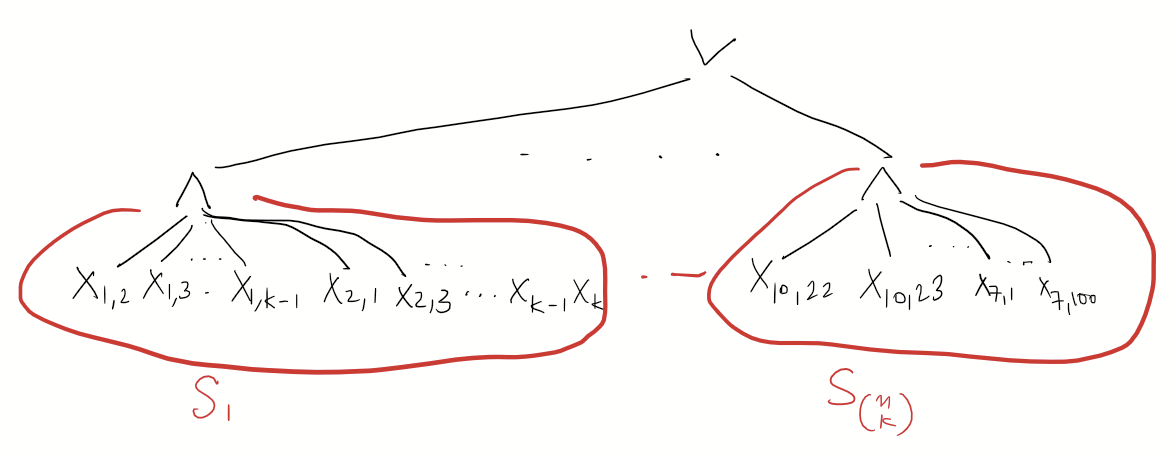
\includegraphics[width=0.75\linewidth]{images/k-clique-simple-circuit.png}
    \label{fig:enter-label}
\end{figure}

$S_1, S_2, \ldots, S_{\binom{n}{k}}$ are the $\binom{n}{k}$ subgraphs in $G$ each of size $k$.
Size of this circuit: $O\left(k^2 \cdot\binom{n}{k}\right)$.
\end{trailer}

A  circuit for computing $\operatorname{CLIQUE}  (n, k),$ consisting of an OR gate $\bigvee$ of many  $S_i$'s, each of size $k$ and where each $S_i$ is an AND of the edge variables in $S_i$, as in the example above, is called a \textit{crude-circuit} for CLIQUE($n, k)$. More formally, we have the following. 

\begin{svgraybox}
\textbf{Crude-circuits $CC\left(X_1, \ldots, X_m\right)$ for CLIQUE}.
Let $V$ be a set of nodes and let $X_1,\dots,X_n\in V$ be a collection of subsets of nodes. The \emph{crude-circuit} $CC\left(X_1, \ldots, X_m\right)$ is defined to be 
$\bigvee_{r=1}^m\bigwedge_{i<j \in X_r} x_{ij}$.
Note that the $X_i$'s may have different sizes (and specifically their sizes may be different from $k$).
\end{svgraybox}

Note that $CC\left(X_1, \ldots, X_m\right)(\alpha)=1$, for $\alpha\in\bits^{n\choose 2}$, precisely when in the graph $G$ over the nodes $V$ described by the assignment $\alpha$, at least one of the $X_i$ subgraphs is a clique. 

% We denote by $CC\left(S_1, \ldots, S_{\binom{n}{k}}\right)$ the crude circuit computing the $\bigvee$ of all subgraphs $S_1, \ldots, S_{n\choose k }$.

\begin{note} 
When $k=\omega(\log n)$, $CC\left(S_1, \ldots, S_{n\choose k}\right)$, where $S_1,\dots,S_{n\choose k}$ are all possible subsets of sizer $k$ from the set of $n$ nodes $V$, is of \emph{exponential size}.
\end{note}

The following theorem shows this naive monotone circuit cannot be improved much.

\begin{figure}
    \centering
    
\includegraphics[width=0.3\linewidth]{images/RAZBOROV_Alexander.jpeg}
    \caption{Alexander Razborov. Creator: Kozloff, Robert | Credit: Photo by Robert Kozloff.
Copyright: The University of Chicago}
    \label{fig:enter-label}
\end{figure}

\begin{svgraybox}
\begin{theorem}[Razborov \cite{Razb85}]\label{thm:razborov} Let $k=\sqrt[4]{n}$. Then, every monotone circuit computing CLIQUE$(n, k)$ has size $2^{\Omega(\sqrt[8]{n})}$.
\end{theorem}
\end{svgraybox}
That is, there exists a constant $c$ such that  for large enough $n \in \mathbb{N}$, if $C_n$ computes CLIQUE$(n,k)$ then $\left|C_n\right| \geq 2^{c \cdot \sqrt[8]{n}}$.


The rest of this chapter aims to prove this theorem. \textbf{Our exposition is taken from Papadimitriou's textbook} \cite{Pap94}.


%Recall: a crude circuit is a big OR of cliques, each computed as a big AND.



\paragraph{Approximation Method}

We first provide an overview of the approach we take to prove \Cref{thm:razborov} which is called \emph{the approximation method}. 
We shall describe a way of approximating any \textbf{monotone} circuit for $\operatorname{CLIQUE}({n}, {k})$ by a crude circuit, namely a big OR of cliques, as follows.

\begin{enumerate}
    
\item  Given a monotone circuit C , we shall construct a crude circuit ${CC}({X} 1, \ldots, {Xm})$ for some m and $\left|{X}_{{i}}\right| \leq l$ (for some $l$, all ${i}=1, \ldots, {m}$ ), that approximates $\operatorname{CLIQUE}({n}, {k})$ with \textbf{precision} that is dependent on the number of gates in $C$.

\item I.e., if the precision is not good, namely the crude circuit ${CC}({X} 1, \ldots, {Xm})$ for CLIQUE (n,k) we end up with makes \textit{many errors} on the CLIQUE ( $n, k$ ) function (i.e., says "NO" on an input that has a k-clique, and "YES" on an input that has no k-clique), it means that the circuit $C$ has \textit{many gates}, and vice versa.\label{it:approximation-b}

\item We show that every crude circuit ${CC}({X}_1, \ldots, {X_m})$ ($|{X}_i| \leq l$ for some $l$, for all $i=1, \ldots, m$ ), ought to make \textit{exponentially many errors} on the function $\operatorname{CLIQUE}(n, k)$. From \ref{it:approximation-b} above we conclude that the number of gates in C was exponential.

\end{enumerate}


The \textbf{approximation} (i.e., construction of a crude circuit for CLIQUE(${n},{k})$ given the circuit $C$) will proceed in steps, one step for each gate of the monotone circuit:

\begin{enumerate}
    
\item If $C$ is a monotone circuit computing $\operatorname{CLIQUE}({n}, {k})$ we can \textit{approximate} any gate OR or AND in $C$ with a crude circuit.

\item Each such approximation step introduces rather few errors (false positives and false negatives).
\end{enumerate}


\section{Proof of monotone circuit lower bounds}

\begin{trailer}{Parameters \& notation}

Recall we want to compute CLIQUE$(n, k)$
with $n$ the number of nodes in the graph and $k$ the size of a clique within the graph. 
We set:
$$
k=\sqrt[4]{n}.
$$

\begin{svgraybox}\textbf{Goal}: Show that every monotone circuit computing $\operatorname{CLIQUE}(n,k)$ has size at least $2^{c \sqrt[8]{n}}$ for some constant $c$ (for sufficiently large $n$).
\end{svgraybox}

$$
\begin{aligned}
& l=\sqrt[8]{n} \\
& p \approx \sqrt[8]{n} \\
& M=(p-1)^l \cdot l! & \approx(\sqrt[8]{n}-1)^{\sqrt[8]{x}} \cdot(\sqrt[8]{n})! \\
& & \leq(\sqrt[4]{n})^{\sqrt[8]{n}}
\end{aligned}
$$


Each crude-circuit we use in the approximation is:

$$
C C\left(x_1, \ldots, x_m\right)
$$

for $m \leqslant M$ and $\left|X_i\right| \leqslant l, \forall i \in[m]$.

\end{trailer}

\bigskip 

\newpage
 

% Enable watermark from this point onward
\SetWatermarkText{DRAFT}

- The approximation of the monotone circuit $C$ that computes $\operatorname{CLIQUE}(n, k)$ is done by induction on the size of $C$, ie., number of $\lor, \wedge$ gates in $C$.


- Comment: Such induction is also called ``Induction on the structure of $C$''.

- Such induction proceeds as follows: 


\para{Base Case} $|C|=1$, ie., $C$ consists of only a single input gate $g_{ij}$. Recall $g_{i j}$ is an input gate denoting whether $(i, j) \in E$, for $i, j \in V$.
That is, if there is an edge between $i$ and $j$ in the input graph $G$.

This is an easy case: We need to show a crude cat $\operatorname{CC}\left(X_1, \ldots, X_m\right)$ with $m \leqslant M$ and $\left|X_i\right| \leqslant l \quad \forall i \in[m]$ that
approximates $g_{i i}$ (without introducing too many errors; We shall count precisely the number of potential errors later).
But the circuit $C C(\{i, j\})=g_{i j}$ by definition. (Hence, no errors here!)


\para{Induction Step}
Given two crude circuits
$\operatorname{CC}(\mathcal X)$ and 
$\operatorname{CC}(\mathcal Y) 
$, with $\mathcal{X}=\{X_1, \ldots, X_m\}$, 
$\mathcal{Y}=\{Y_1, \ldots, Y_{m^{\prime}}\}$, $m\le M$, and $\left|X_i\right| \leq \ell $, for all $i$, $m'\le M $ and $\left|Y_i\right| \leq \ell$, for all $i$.


We wish to construct another crude circuit  for computing $CC(\mathcal{X}) \vee CC(\mathcal{Y})$, and $\operatorname{CC}(\mathcal X) \wedge 
\operatorname{CC}(\mathcal Y)$.

\case{1}
$\lor$-gate.

\textit{Naive attempt}: $\operatorname{CC}(\mathcal X)
\lor \operatorname{CC}(\mathcal Y)$ is approximated by $\operatorname{CC}(\mathcal X \cup \mathcal Y)$. That is, $\operatorname{CC}\left(X_1, \ldots, X_m, Y_1, \ldots, Y_m\right)$. At first glance this is a good solution because it does not introduce any errors (why?). But there is a \textit{problem}: what if $m+m^{\prime}>M$?


\textit{Solution}: We need to cleverly \emph{reduce} the number of sets $X_1, \ldots, X_m, Y_1, \ldots, Y_{m^{\prime}}$. To do this we use a combinatorial lemma called The Sunflower Lemma.





\section{The Sunflower Lemma}

\begin{figure}
    \centering
        \includegraphics[width=0.75\linewidth]{images/sunflower-lemma.png}
    \caption{From https://theorydish.blog/2021/05/19/entropy-estimation-via-two-chains-streamlining-the-proof-of-the-sunflower-lemma/ by Lunjia Hu}
    \label{fig:enter-label}
\end{figure}



%Let $U$ be some universe, namely a set of elements (e.g., nodes). Let $Z=\{Z_1,\dots,Z_M\}$ be a family of sets from the universe, i.e., $Z_i\subseteq U$, for each $i$, with $M$ some natural number. %We call the family $P$ a \emph{sunflower} if  $\left\{P_1, \ldots, P_p\right\}$ called \emph{petals}, each $\left|P_i\right| \leqslant \ell$ where $\ell=\sqrt[8]{n}$, such that all pairs $P_i \neq P_j$ in the family share the \emph{same} intersection, called the \emph{core} of the sunflower. In other words, there is a set  $ P_i\cap P_j = Core$

\begin{svgraybox}
\begin{definition}[Sunflower] Let $U$ be some universe, namely a set of elements (e.g., nodes). Let $P=\{P_1,\dots,P_p\}$ be a family of distinct sets from the universe, i.e., $P_i\subseteq U$, for each $i$, with $p$ some natural number. 
We call the family $P$ a \emph{sunflower} if each all pairs $P_i \neq P_j$ in the family $P$ share the \emph{same} intersection, called the \emph{core} of the sunflower.
In other words, there is a (possibly empty) set $\mathrm{core}\subseteq U$, such that for all $i\neq j$,  $ P_i\cap P_j = \mathrm{core}$.
If $P$ is a sunflower we call the $P_i$'s the \emph{petals} of the sunflower $P$.
\end{definition}
\end{svgraybox}
Note: It's okay if the core is the empty-set! This means all petals are (pairwise) disjoint.


\begin{svgraybox}
\textbf{Sunflower Lemma} (Erd\"os-Rado): For every $\ell, p$, let $Z$ be a family of more than $M=(p-1)^\ell \cdot \ell!$ non-empty sets each of size $\leqslant \ell$ (over some universe $U$). Then, $Z$ contains a sunflower of size $p$. In other words, $Z$ contains $p$ sets $\left\{P_1, \ldots, P_p\right\}$, each $P_i$ has size $\leqslant \ell$, and the intersection of every pair $P_i \neq P_j$ is fixed: $P_i \cap P_j=P_{i'} \cap P_{j'}$, for all $i \neq j \neq i' \neq j^{\prime}$.
\end{svgraybox}



\begin{proof}[Proof of the Sunflower Lemma]
By induction on $\ell$.

\Base  $\ell=1$. Thus the statement we need to show is that $p$ different singletons form a sunflower. Which is true (the core is $\varnothing$ ).


\induction $\ell>1$. Consider a family $D \subseteq Z$ of pairwise disjoint sets that is maximal in the sense that if we add any new set in $Z$ to the family $D$, the sets in $D$ are not pairwise disjoint anymore. That is, every set in $Z \backslash D$ intersects some set in $D$.

\case 1 If $D$ contains $\geq p$ sets then $D$ is a sunflower with empty core, and we are done.

\case 2 Otherwise, let $E$ be the \emph{union} of all sets in $D$.
Since $|D|<p$, i.e., $D$ contains less than $p$ sets, and each set in $D$ has size $\le \ell$, we know that $|E| \leqslant(p-1)\cd\ell$.

\medskip 

Moreover, $E$ intersects every set in $Z$ by assumption.
Since $Z$ has more than $M$ sets by assumption, and each set intersects some element of $E$, there exists an element $d \in E$ that intersects $>\frac{M}{(p-1) l}=(p-1)^{l-1} \cdot(l-1)!$ sets in $Z$.


\begin{remark}
If a set $E$ intersect all sets in a family of sets $X_1, . ., X_M$ then there is an element in $E$ that appears in $\geq \frac{M}{|E|}$ sets $X_i$.
Otherwise, each element in $E$ appears in $<\frac{M}{|E|}$ sets $X_i$. Thus, $E$ intersects $<|E| \cdot \frac{M}{|E|}=M$ sets $X_i$, which is a contradiction to the assumption.
\end{remark}


Consider

$$
Z^{\prime}:=\{z \backslash\{d\} \mid z \in Z \text { and } d \in z\} .
$$


We know that $Z^{\prime}$ contains more than $M^{\prime}=(p-1)^{l-1} \cdot(l-1)!$ sets.
By \emph{induction hypothesis} (since $M^{\prime}$ is "$M$ with $\ell$ decreased by one"), $Z^{\prime}$ contains a sunflower denoted $\left\{P_1, \ldots, P_p\right\}$ with $\left|p_i\right| \leq \ell-1$, for all $i$.
Hence, $\left\{P_1 \cup\{d\}, \ldots, P_p \cup\{d\}\right\}$ is a sunflower in $Z$.
This concludes the Sunflower Lemma's proof.
\end{proof}



Approximating $O R$ and AND using Plucking
- By the Sunflower Lemma, every family of $\geq M$ nonempty sets, each of cardinality $\leqslant l$, then we can find a sunflower in it with $l=\sqrt[3]{n}(p \approx \sqrt[3]{n}) M=(p-1)^l \cdot \ell!$.
- Plucking a sunflower: replacing all petals by their core. 4 sets

Corollary: If we have $>M$ sets in a family, by repeated plucking we can reduce the number of sets to $\leq M$ (if we cant apply plucking. anymore we know by the Sunflower Lemma that the number of sets is $\leqslant M$ ).
pluck (z): the result of repeated plucking of a family of sets $Z$, until $|Z| \leqslant M$.
Definition (Approximate OR and AND): foxily of sets The approximate $-V$ of two crude -circuits $C C(x)$ and $\operatorname{cc}(y)$ is: $\operatorname{cc}($ pluck $(x \cup y))$.

The approximate $-\Lambda$ of $C C(x)$ and $C C(Y)$ is: $\operatorname{cc}\left(\right.$ pluck $\left\{X_i \cup Y_j:\left|X_i \cup Y_j\right| \leqslant l\right.$ and $\left.\left.X_i \in \chi, Y_j \in Y\right\}\right)$





False Positives \& False Negatives

We shall now show that $V$ and $\Lambda$-approximators are good, in the sense that they introduce few errors!

Out of all possible inputs to a cat computing Clique ( $n, k$ ) (for $k=\sqrt[4]{n})$, the ne are:
Accept-instances: $G=(V, E)$ is a graph on $n$ modes that contains a $k$-clique.
Reject-instances: $G=(V, E)$ is a graph on $n$ nodes that does not contain a $k$-clique.
We shall restrict attention $t_0$ only subsets of Accept and Rejed instances. This will be sufficient for the proof (it's more convenient that way). Thus, our focus is on "extreme" cases of inputs:



- Positive-lnputs: $G=(v, E)$ has $x$ nodes and a $k$-clique ( $k$ nodes $w /$ all edges between them); while no other edge exist in $G$.

\begin{figure}[H]
    \centering
    \includegraphics[width=.5\linewidth]{images/clique1.png}
    \caption{Enter Caption}
    \label{fig:enter-label}
\end{figure}


There are $\binom{x}{k}$ positive-inputs, each one is dearly an accept input to $\operatorname{CUQ} \cup E(n, k)$.
- Negative Inputs: $G=\left(v_1 E\right)$ has $n$ nodes and $(k-1)$-colouring (independent sets). In other words, nodes $V$ are coloured by some $k-1$ colours (one colour for each independent set [ie., set of nodes w/ no edge between them]). And all edges between notes w/ different colours.



\begin{figure}[H]
    \centering
    \includegraphics[width=.6\linewidth]{images/clique2.png}
    \caption{Enter Caption}
    \label{fig:enter-label}
\end{figure}



Note: 1) There are $(k-1)^n$ negative -inputs. (We count twice two identical graphs w/ colours interchanged.)
2) A $(k-1)$-colouring is a negative-input for $\operatorname{CUQUE}(n, k)$ because a $k$-clique cannot be coloured by $k-1$ colours.
3) In fact, even a single edge added to a $(k-1)$-colouring will make the graph contain a k-clique!




$V$-approximator of $\operatorname{CC}(x) \vee \operatorname{CC}(y)$ introduces
1) a false negative:

A k-clique $G=(v, E)$ s.t.: $(\operatorname{cc}(x) \operatorname{vcc}(y))(G)=1$
2) a false positive:
$\operatorname{cedpluck}(x \cup y)(G)=0$
$V$-aterosimator
$A(k-1)$-coburing $G=(v, E)$ s.t.

$$
\begin{aligned}
& (\operatorname{cc}(x) \vee \operatorname{cc}(y))(G)=0 \\
& \frac{\operatorname{cc}(p l u c k(x \cup y))(G)}{V \text {-approvinator }}=1
\end{aligned}
$$


1 -apporimator of $\operatorname{CC}(x) \wedge \operatorname{CC}(y)$ introduces
1) a false negative:

A k-clique $G=(v, E)$ s.t: : $(\operatorname{cc}(x) \wedge \operatorname{cc}(y))(G)=1$
2) a false positive: $c c\left(P \mid\right.$ luck $\left.\left\{x_i\left|y_i:\left|x_i \cup y_i\right| \leq l, x_i \in X, y_i \in\right\}\right\}\right)=0$

$$
\left.c c\left(p l u c k\left\{x_i \cup Y_j:\left|x_i \cup y_0\right| \leq l, x_i \in \chi, y_i \in\right\}\right\}\right)=1
$$


Lemma 1: Each approximation step introduces at most $M^2 \cdot \frac{(k-1)^n}{2^p}$ false positives.

Lemma 2: Each approximation step introduces at most $M^2 \cdot\binom{n-l-1}{k-l-1}$ false negatives.

Proof of monotone Pkt lower bound from these lemmas. CLAIM: Every crude-ctt CC $\left(X_1, \ldots, x_m\right) w /$ $\left|x_i\right| \leq l$ and $m \leqslant M$ is either identically 0 (and thus is wrong on all positive-instances), or outputs 1 on at least half of the negative -instances.
Proof: If $\operatorname{CC}\left(x_1 \ldots x_m\right) \neq 0$, then it accept's at least those graphs $G$ that have cliques on at least one of the sets $X_i$, for some $i$. The size of $X_i$ is $\leqslant l<k$, thus many graphs $G$ that are not $k$-cliques still have e-cliqnes



cont.
Let's count how many such graphs exist, using probability. Consider a graph $G=(V, E)$; assign randomly (and independently) from among $(k-1)$ colours to the modes of $G$. Let $v_1 \neq v_2 \in V$ be two nodes.

$$
\operatorname{Pr}\left[\text { colour of } v_1=\text { colour of } v_2\right]=\frac{1}{k-1}
$$


Denote by $R\left(X_i\right)$ the evert that in the random colouring to $G$, there exists a pair of nodes with the same colour in $X_i$
Then, $\operatorname{Pr}\left[R\left(x_i\right)\right] \leqslant \frac{\binom{x_i \mid}{ 2}}{k-1} \leqslant \frac{\binom{l}{2}}{k-1} \leqslant \frac{1}{2}$.
there are $\binom{\mid x_i i}{2}$ pairs
of nodes in $X_i$. We use
the union bound.
This means that out of all negative-instances to CLIQUE $(n, k)$ (namely, all ( $k-1)$-colouring of a graph w/ $n$ nodes), at least half of them are going to colour $X_i$ w/ different colours. Hence, for these negative -instance, there will be edges between all nodes in $X_i$, and thus $\left(C\left(x_1, \ldots, x_m\right)(G)=1\right.$ for each of these negative instances $G$.




We are now ready to conclude the main result.
Recall: $l=\sqrt[8]{n}$ and
Let $p=\sqrt[8]{n} \cdot \log n$. Thus, $M_i=(p-1)^l \cdot l!<\left(n^{\frac{1}{3}}\right)^{\sqrt[8]{n}}$, for large
- Let $C$ be a monotone cat computing CLQUE $(n, \sqrt[4]{n})$.
- We apply the approximators at each gate of $C$ iteratively.
- The output gate of $C$ thus is written as a $\operatorname{CC}\left(x_1, \ldots, x_m\right)$ for some $m \leqslant M$ and $\left|x_i\right| \leqslant l$.
- Based on the above, we have two cases:

Case 1: $\operatorname{cc}\left(x_1, \ldots, x_m\right) \equiv 0$.
Thus, the number of false negatives introduced is the total of all possible positive-instance, namely all possible $k-c$ cliques: $\binom{n}{k}$.
Thus,

$$
|C| \geq \frac{\binom{n}{k}}{\operatorname{lemmax}^2\binom{n-l-1}{k-l-1}} \geq \frac{1}{M^2}\left(\frac{n-l}{k}\right)^l \geq n^{c \sqrt[8]{n}},
$$


Case $2: \operatorname{CC}\left(x_1, \ldots, x_n\right)$ has at least $\frac{1}{2}(k-1)^n$ false positives (half of $(k-1)$-colourings).
By Lemma 2: $|c| \geq \frac{\frac{1}{2}(k-1)^n}{M^2 \frac{(k-1)^n}{2^p}}=\frac{2^p}{2 \cdot M^2}>n^{c \cdot 8} n$, for $c=\frac{1}{3}$.



Lemma 1: Each approximation step introduces at most $M^2 \frac{(k-1)^n}{2^p}$ false positives.

Pe of F: Case 1: OR-approximator
We start with $\overline{C C}\left(x_1, \ldots, x_m\right)$ and $\operatorname{CC}\left(y_1, \ldots, y_{m_m}\right)$ and consider a false positive introduced by

$$
\operatorname{cc}\left(\text { pluck }\left(X_1, \ldots, X_m, Y_1, \ldots, Y_{m^{\prime}}\right)\right) \text {. }
$$


That is, a $G=(v, E)$ s.t.,

$$
\operatorname{cc}\left(x_1, \ldots, x_m\right)(G)=0, \quad \operatorname{cc}\left(y_1, \ldots, y_m\right)(G)=0
$$

and

$$
\operatorname{cc}\left(\operatorname{pluck}\left(X_1, \ldots, X_m, Y_1, \ldots, Y_{m^{\prime}}\right)\right)(G)=1 .
$$


We consider each plucking involved in (2), and bound from above the number of false positive introduced by this plucking. (Note this is the only reason a false positive can be introduced.)


 - Consider a single plucking : replace sunflower $\left\{z_1, \ldots, z_p\right\}$ by its core $Z$.

By (1): $Y_i^{\prime} s \& X_i^{\prime} s(\&, ' s)$
are all hon-cliques
Thus, by (2)
$Z$ is a clique
and every petal $z_i$
has two nodes w/ the $\frac{\text { same colour! }}{L \operatorname{bg}(1)}$



\begin{figure}[H]
    \centering
    \includegraphics[width=.6\linewidth]{images/clique3.png}
    \caption{Enter Caption}
    \label{fig:enter-label}
\end{figure}


- We count the number of such colourings.
- We do this probabilistically:

Choosing a $(k-1)$-colouring of the nodes randomly and independently, what's the probability every $z_i$ has repeated colours but $z$ does not?
- As before, let $R(X)$ be the probability that $X$ has repeated colours.


$\qquad$ As before, let $R(X)$ be the probability that $X$ has repeated colours.

$$
\operatorname{pr}\left[R\left(z_1\right) \wedge \ldots \wedge R\left(z_p\right) \wedge \neg R(z)\right] \leqslant \operatorname{pr}\left[R\left(z_1\right) \wedge \ldots \wedge R\left(z_p\right) \mid \neg R(z)\right]$$

$$
\begin{aligned}
& =\prod_{i=1}^p \operatorname{Pr}\left[R\left(z_i\right) \mid \neg R(z)\right] \\
& \leqslant \prod_{i=1}^p \operatorname{Pr}\left[R\left(z_i\right)\right]
\leqslant \frac{1}{2^p}
\end{aligned}
$$

$$
\operatorname{Pr}[A \| B]=\operatorname{Pr}[A \mid B] \cdot \operatorname{Pr}[B]
$$


Li's don't have common nodes, except those in $Z$.

We've seen before that

$$
\operatorname{Pr}[R(x)] \leqslant \frac{1}{2}
$$

Probability of repetition of colours is increased if we doit restrict ourselves to colourings w/ no repetitions in $z \subseteq Z_i$.


Finally, since the approximation step entails up to $\frac{2 M}{p-1}$ pluckings (each plucking decreases the number of sets by $\mathrm{p}-1$, and there are no more than 2 M sets when we start), the lemma holds for the OR approximation step: because e

$$
M^2 \cdot \frac{(k-1)^n}{2^p} \geq \frac{2 M}{p-1} \cdot \frac{(k-1)^n}{2^p}
$$


Cont. of proof of Lemma 1

Consider now an AND approximation step of crude circuits $C C(x)$ and $C(y)$. It can be broken down in three phases: First, we form $C C(\{X \cup Y: X \in \chi, Y \in Y\})$; this introduces no false positives, because any graph in which $X U Y$ is a clique must have a clique in both and $Y$, and thus it was accepted by both constituent crude circuits. The second phase omits from the approximator circuit several sets (those of cardinality larger than $\ell$ ), and can therefore introduce no false positives. The third phase entails a sequence of fewer than $\mathrm{M}^2$ plucking, during each of which, by the analysis of the OR case above, at most $2^{-\mathrm{P}}(\mathrm{k}-1)^{\mathrm{n}}$ false positives are introduced. The proof of the lemma is complete: because at total we introduced $\leq M^2 \cdot \frac{(k-1)^n}{2^p}$ false positives




Lemma 2: Each approximation step introduces $\leqslant M^2\binom{n-l-1}{k-l-1}$ false negatives.
PRoOF:
Case $V_{:}$a false negative:
A $k$-clique $G=(v, E)$ st.: $(\operatorname{cc}(x) \vee \operatorname{ccc}(y))(G)=1$ (

$$
\underbrace{\operatorname{colpluck}(x \cup y)(G)}_{V \text {-aproximator }}=0
$$


This is impossible, because plucking only deletes sets and make them smaller; hence if (1) holds then (2) cannot.
Case 1:
A false negative:
A $k$-clique $G=(v, E)$ st: : $(\operatorname{cc}(x) \wedge \operatorname{cc}(y))(G)=1$

$$
\left.c\left(P / \mid u c k\left\{x_i \cup Y_j:\left|x_i \cup Y_i\right| \leq l, x_i \in \chi_{,}, Y_i \in\right\}\right\}\right)=0 \text { (2) }
$$


In the first stop we replace $c a(x) \wedge c(y)$ by $C C(\{X \cup Y: x \in X, y \in Y\})$.
Hence, if $G$ is a $K$-clique and both $X$ and $Y$ are each cliques in $G$, it must be that $X \cup Y$ is also a clique in $G(w h y$ ? ). Thus, no false negatives are introduced in this step.


$\frac{\text { (cont.) }}{\text { We next delete all sets } \overbrace{X_i \cup Y_j}^{\text {denoted }} Z}$ larger than $l$. This introduce several false negatives:
All $k$-cliques $G$ that contain $Z$.
We calculate an upper bound on these false negatives: There are precisely $\binom{n-|z|}{k-|z|}$ k-cliques er that contain $z$ (as part of the clique). Since, $|z|>l$, the upper bound on the false negatives introduced by each deletion is $\binom{n-l-1}{k-l-1}$.

Since there are $\leqslant M^2$ deletions of sets, (because $|\chi|=|y|=M$ ), we get that the number of false negatives introduced by $a_n 1$-approximation step is $\leqslant M^2 \cdot\binom{n-t-1}{k-l-1}$.
